\documentclass{rapport}
\usepackage{lipsum}
\usepackage{gensymb}
\usepackage{float}
\usepackage{graphicx} % Pacchetto obbligatorio per le immagini
\usepackage{wrapfig}  % Pacchetto per avvolgere il testo
\usepackage{amsthm} 
\usepackage{amssymb}
\usepackage{cancel}
\usepackage{polynom}

\usepackage{enumitem}
\usepackage[most, theorems]{tcolorbox}
\usepackage{xcolor}
\usepackage[italian]{babel} % lingua italiana

\usepackage[utf8]{inputenc}
\usepackage{pgfplots}
\pgfplotsset{compat=1.18}

\usepackage{tikz}
\newcommand*\circled[2][]{%
  \tikz[baseline=(char.base)]{
    \node[shape=circle,draw=#1,inner sep=1pt] (char) {$\displaystyle #2$};
  }%
}
\usetikzlibrary{patterns}

\usetikzlibrary{arrows.meta}
\usetikzlibrary{matrix, positioning}

\newtcbtheorem{teorema}{Teorema}{
  colback=blue!5!white,
  colframe=blue!75!black,
  enhanced,
  fonttitle=\bfseries,
}{theo}

\newtcbtheorem{definizione}{Definizione}{
    colback=green!5!white, 
    colframe=green!75!black, 
    enhanced,
    fonttitle=\bfseries,
}{def}

\newtcbtheorem{esercizio}{Esercizio}{
    colback=red!5!white, 
    colframe=red!75!black, 
   enhanced,
  fonttitle=\bfseries,
}{es}

\newtcbtheorem{corollario}{Corollario}{
    colback=pink!5!white, 
    colframe=pink!75!black, 
    enhanced,
  fonttitle=\bfseries,
}{corr}

\newtcbtheorem{esempio}{Esempio}{
    colback=purple!5!white, 
    colframe=purple!75!black, 
    enhanced,
  fonttitle=\bfseries,
}{esem}

% \newtheorem{theorem}{Teorema}
% \newtheorem{proposition}[theorem]{Proposizione}
% \newtheorem{corollary}[theorem]{Corollario}
% \newtheorem{lemma}[theorem]{Lemma}

% \theoremstyle{definition}
% \newtheorem{definition}[theorem]{Definizione}
% \newtheorem{axiom}[theorem]{Assioma}
% \newtheorem{example}[theorem]{Esempio}

% \theoremstyle{remark}
% \newtheorem{remark}[theorem]{Remark}
% \newtheorem{note}[theorem]{Note}
\def\mathunderline#1#2{\color{#1}\underline{{\color{black}#2}}\color{black}}
\newcommand{\mathrect}[2]{%
  \fcolorbox{#1}{white}{\strut$\displaystyle #2$}%
}

\title{DataBase} %title of the file

\begin{document}

%----------- Report information ---------

\logo{logos/logo.jpg}
\uni{\textbf{Università degli Studi di Padova}}
\ttitle{Fisica 1} %title of the file
\subject{Fisica1} % Subject name
\topic{Fisica1} % Topic name

\students{Alex Gasparini} % information related to the students

%----------- Init -------------------
        
\buildmargins % display margins
\buildcover % create the front cover of the document
\toc % creates the table of contents

%------------ Report body ----------------



\paragraph{Introduzione}
\addcontentsline{toc}{subsection}{Introduzione a Fisica 1}
\begin{wrapfigure}{r}{4cm}
    \centering
    \includegraphics[width=3.5cm]{img/Galileo.jpg} 
    \caption*{Galileo Galieli}
\end{wrapfigure}
La \textbf{Fisica} è una scienza speriementale che si occupa di sviluppare modelli matematici in grado di descrivere fenomeni naturali e fornire predizioni quantitative. Con questa definizione capiamo che la fisica è una disciplina che si preoccupa di prevedere eventi naturali, usanso dei modelli matematici. Questa concezzione di fisica è relativamente recente, infatti venne idealizzata da \textbf{Galileo Galieli}. Galileo  nato a Pisa il 15 febbraio 1564 e morto l'8 gennaio 1642, portò ad un cambiamento radicale nella scena scientifica di all'ora: usare un approccio \textbf{qualitativo}, e non \textbf{quantitativo} come si faceva fino a quel momento. 

Prima di Galileo si usava un approccio basato sui sensi, facciamo un esempio per capire meglio: per indicare la temperatura atmosferica si diceva "è molto caldo", "è freddo", "è mite" ecc... Pertanto non si usava una misura precisa ed universale, e questo poteva portare a delle ambiguità perchè ognuno percepisce i sensi a modo suo, e quindi ciò che è caldo per me, per te potrebbe essere tiepido o addirittura freddo. 

Galileo riconobbe questo problema e decise di misurare i fenomeni basandosi sui strumenti di misura, così chiunque possa avere un valore oggettivo, senza l'uso dei sensi. Se questo a primo impatto vi sembra un qualcosa di ovvio è proprio perchè questa idea che ha avuto Galileo è la basa fondante della fisica odierna. 

In questo corso vedremo due macro-argomenti: \textbf{Meccanica} e \textbf{Termodinamica}. La meccanica è la disciplina che si occupa di studiare i moti mentre la termodinamica studia come gli scambi di energia sotto forma di calore. La prima che vedremo è la meccanica che si divide in due categorie: \textbf{Cinematica} e \textbf{Dinamica}. La cinematica si occupa di studiare come avvengono i moti, e quindi di riuscire a predirre i moti conoscendo le condizioni iniziali, mentre la dinamica studia il perchè avvengono i moti, andando ad analizzare le relazioni tra causa e concausa.

\begin{wrapfigure}{l}{4cm}
    \centering
    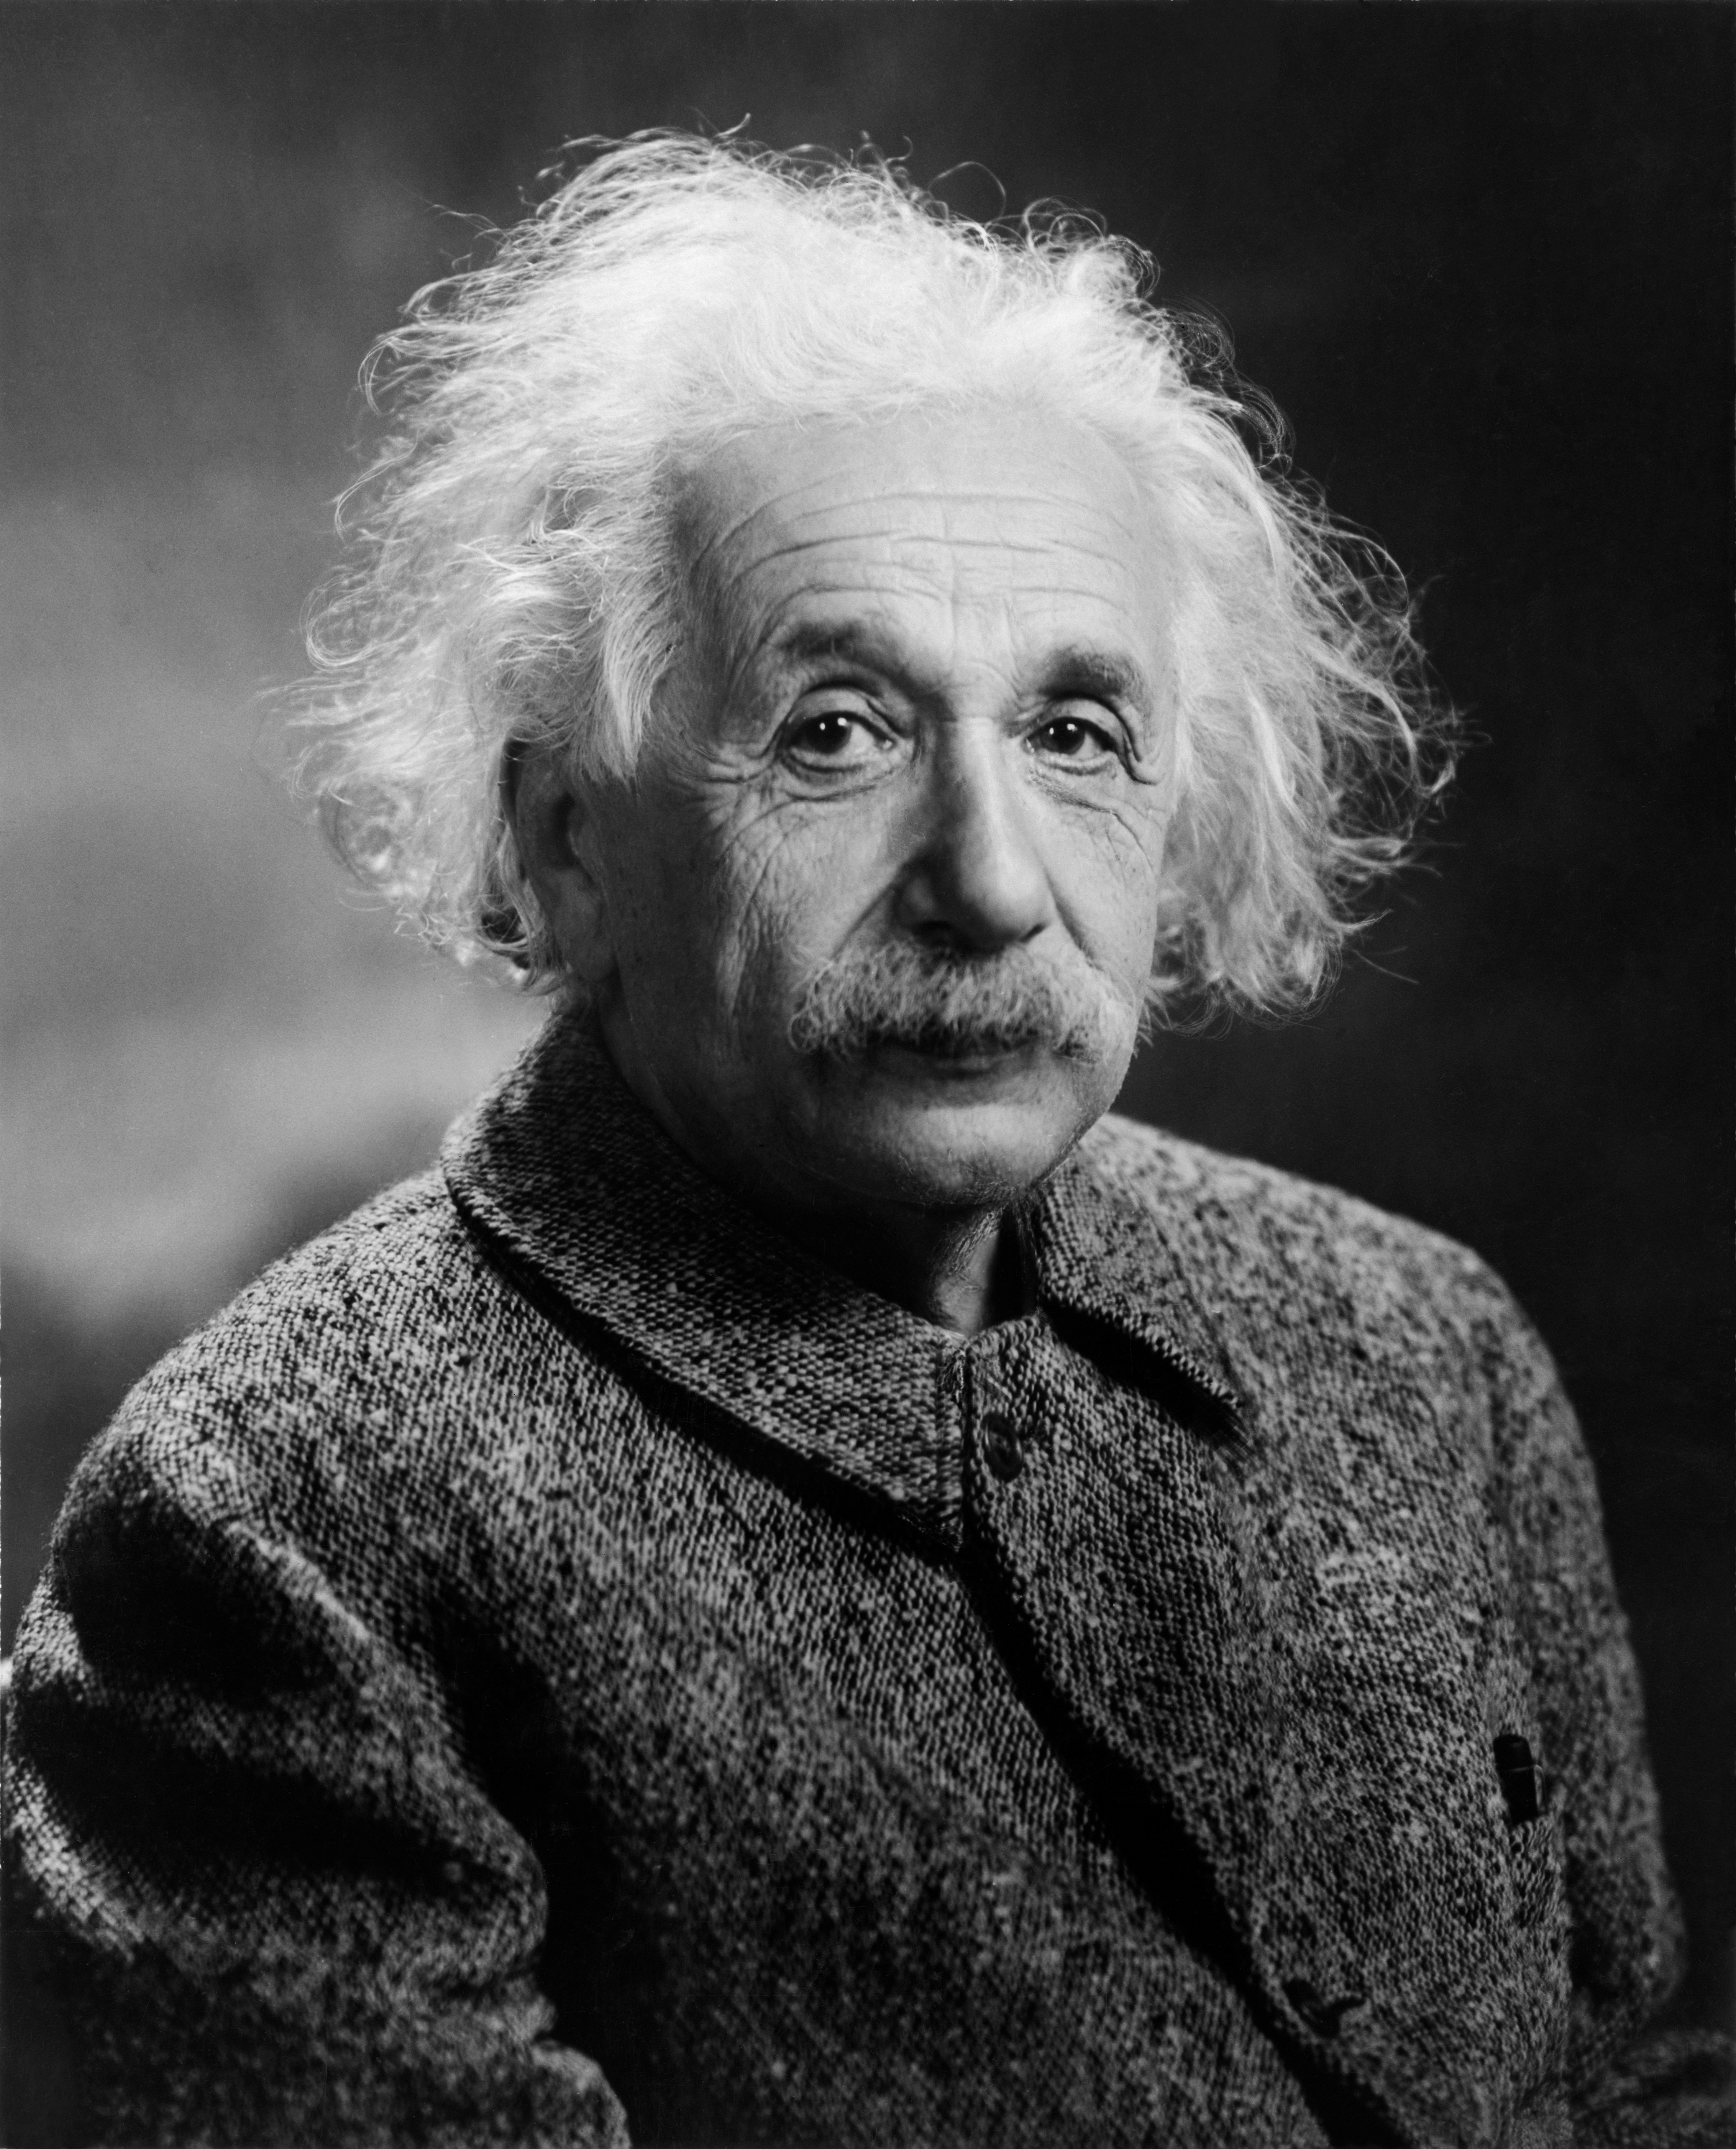
\includegraphics[width=3.5cm]{img/Einstein.jpg} 
    \caption*{Albert Einstein}
\end{wrapfigure}

Un concetto fondamentale da capire e mettere in chiaro è che per questo corso noi consideremo il tempo come variabile indipendente, e che quindi relazioneremo tutte le altre grandezze fisiche rispetto al tempo, questo perchè fino ad un centinaio di anni fa si credeva che il tempo fosse uguale per tutti, e quindi tutti possono replicare gli esperimenti ed avere gli stessi risultati.

Questo però fu smentito nel 1905 da \textbf{Albert Einstein} con la \textbf{Relatività Ristretta}, scoprendo che il tempo è relativo e che quindi a parità di esperimeno si possono misurare grandezze diverse. Per fortuna, gli effetti che ha scoperto Einstein sono rilevanti solo a velocità prossime alla luce, quindi nei nostri casi studio tratteremo esempi più concreti, di oggetti che difficilmente raggiungono velocità elevate, pertanto questo ci permette di tralasciare gli effetti relativistici e dare per assodato che il tempo è unico per tutti gli osservatori.

\section{Meccanica: Cinematica}

\begin{definizione}{Legge Oraria}{}
 \addcontentsline{toc}{subsection}{Definizione di Legge Oraria}
    Una \textbf{Legge Oraria} è una qualsiasi funzione che descrive lo spazio (usa sola dimensione) rispetto al tempo. Un esempio può essere 

    \begin{equation*}
      x(t) = 2t - t^2
    \end{equation*}

    con $x$ si intende la posizione e $t$ il tempo
\end{definizione}

La legge oraria è fondamentale perchè ci permette di analizzare interamente il moto e sopratutto ci permette di disegnare il \textbf{grafico spazio-tempo}, altro non è che il grafico della funzione legge oraria. Ad esempio prendendo l'esempio $x(t) = 2t-t^2$ possiamo disegnare il grafico ed abbiamo  
\begin{figure}[htbp]
    \centering
    \begin{tikzpicture}
        \begin{axis}[
            axis lines = middle,
            xlabel = {$t$}, 
            ylabel = {$x(t)$}, 
            xmin = 0, xmax = 2.7,
            ymin = -0.5, ymax = 1.2, 
            domain = 0:2.2,        
            samples = 100,         
            grid = none,          
            width=7cm, height=5cm, % Ho aumentato un po' l'altezza per chiarezza
            xlabel style={anchor=west}, 
            ylabel style={anchor=south},
            % --- AGGIUNTA IMPORTANTE ---
            % Definiamo quali numeri mostrare esattamente sugli assi
            % per far apparire 1.5 e 0.75
            xtick={0, 0.5, 1, 1.5, 2, 3},
            ytick={-2, -1, 0, 0.75, 1, 2},
            % Opzionale: formatta il 0.75 per non sovrapporsi troppo
            yticklabels={-2, -1, 0, \footnotesize$0.75$, 1, 2}
            % ---------------------------
        ]
        
        % La funzione principale
        \addplot [
            thick,
            blue,
        ] {2*x - x^2};

        % --- LINEE TRATTEGGIATE ---
        
        % 1. Proiezione del VERTICE (1,1)
        % Disegna una linea grigia, sottile e tratteggiata
        % Dall'asse t (1,0) -> al punto (1,1) -> all'asse x(t) (0,1)
        \draw[dashed, thin, gray] (1,0) -- (1,1) -- (0,1);
        
        % 2. Proiezione del punto a t=1.5 (che corrisponde a x=0.75)
        % Dall'asse t (1.5, 0) -> al punto (1.5, 0.75) -> all'asse x(t) (0, 0.75)
        \draw[dashed, thin, gray] (1.5,0) -- (1.5, 0.75) -- (0, 0.75);

         \draw[dashed, thin, gray] (0.5,0) -- (0.5, 0.75);
        % (Opzionale) Aggiunge due pallini sui punti di intersezione per evidenziarli
        \addplot[mark=*, mark size=1.5pt, gray] coordinates {(1.5, 0.75)};
        \addplot[mark=*, mark size=1.5pt, gray] coordinates {(0.5, 0.75)};
        \addplot[mark=*, mark size=1.5pt, gray] coordinates {(1,1) };

        % --------------------------

        \end{axis}
    \end{tikzpicture}
\end{figure}

Con questo grafico possiamo capire varie informazioni, in primis dove si trova la funzione in un determinato punto. Ad esempio se io volessi trovare dove si trova l'oggetto descritto da questa legge oraria al tempo $t=1s$, basta che calcoliamo $x(1)=1m$. Pertanto dopo $1s$ abbiamo scoperto che il nostro oggetto è a $1m$ dall'inizio.  Possiamo però fare anche un ragionamento contrario, ovvero chiederci a che tempi il nostro oggetto è a $0.75m$ dall'inizio. Quindi dobbiamo risolvere l'equazione $x(t)=0.75$, che porta alle soluzioni $t_1=0.5s $ e $t_2 = 1.5s$, il che vuol dire che il nostro oggetto è a $0.75m$ dall'origine in 2 instanti, questo fa presagire che il nostro oggetto sia andato avanti e poi sia tornato indietro.

\textbf{N.B.} nei grafici spazio-tempo non ha senso disegnare il semiasse positivo delle ascisse, dato che implicherebbe un tempo negativo, quindi per convenzione si è deciso di partire con $t=0s$. 


\begin{definizione}{Velocità Media}{}
\addcontentsline{toc}{subsection}{Definizione di Velocità}
  Definiamo la \textbf{velocità media} di un moto nell'intervallo $[t_0, t_1]$, con $t_1 > t_0$, con la seguente espressione 
  \begin{equation*}
    v_m = \dfrac{\Delta x(t)}{\Delta t} = \dfrac{x(t_1) - x(t_0)}{t_1-t_0}
  \end{equation*}
  con $v_m$ si intende la velocità media e $x(t)$ la legge oraria del moto.
\end{definizione}

Usando l'esempio di prima possiamo calcolare la velocità media nell'intervallo $[1,1.5]$

\[
v_m = \dfrac{x(t_1) - x(t_0)}{t_1-t_0} = \dfrac{0.75 - 1}{1.5-1}= -0.5
\]

Spesso però più che la velocità media a noi ci interessa la \textbf{velocità istantanea}.

\begin{definizione}{Velocità Istanta}{}
  Definiamo la \textbf{velocità istantanea} di un moto come il limite della velocità media nell'intervallo $[t, t + \Delta t]$, con $\Delta t>0$, per $\Delta t \to 0$.
  \[
  v(t) = \lim_{\Delta t \to 0} \dfrac{x(t+\Delta t)-x(t)}{\Delta t}
  \]

  Ma questo riconosciamo che è la definizione di derivata, quindi possiamo dire che 
  \[
  v(t) = \dfrac{d x(t)}{dt}=\dot{x}(t)
  \]
  in fisica spesso è usata anche la notazione $\dot{x}(t)$ per indicare la derivata di una funzione rispetto al tempo.
\end{definizione}

Quindi rimanendo all'esempio di prima, possiamo calcolare la velocità istantanea
\[
v(t) = \dfrac{d x(t)}{dt} = \dfrac{d}{dt} \left(2t-t^2\right) = 2-2t
\]
La velocità istantanea la possiamo interpretare come la velocità che è segnata dal tachimetro in una macchina che sta eseguente il moto descritto dalla legge oraria $x(t)$. Quindi con il solito esempio possiamo calcolare la velocità in qualsiasi momento, e per esempio se io volessi sapere a che velocità stà andando il nostro oggetto al momento $t=2s$ basta calcolare $v(2) =  -2m/s$. Il meno sta ad indicare la direzione nel quale stiamo percorrendo, ed in questo caso è come se stessimo facendo la retromarcia dato che il segno meno sta a dire che stiamo andando in direzione opposta rispetto a dove punta l'auto.

\begin{definizione}{Accelerazione Media}{}

\addcontentsline{toc}{subsection}{Definizione di Accelerazione}
  Definiamo l'\textbf{accelerazione media} di un moto nell'intervallo $[t_0, t_1]$, con $t_1 > t_0$, con la seguente espressione 
  \begin{equation*}
    a_m = \dfrac{\Delta v(t)}{\Delta t} = \dfrac{v(t_1) - v(t_0)}{t_1-t_0}
  \end{equation*}
  con $a_m$ si intende l'accelerazione media e $v(t)$ la velocità istantanea del moto.
\end{definizione}

Come prima, più che l'accelerazione media a noi ci interessa l'accelerazione istantanea.

\begin{definizione}{Accelerazione Istanta}{}
  Definiamo l'\textbf{accelerazione istantanea} di un moto come il limite dell'accelerazione media nell'intervallo $[t, t + \Delta t]$, con $\Delta t>0$, per $\Delta t \to 0$.
  \[
  a(t) = \lim_{\Delta t \to 0} \dfrac{v(t+\Delta t)-v(t)}{\Delta t} = \dfrac{d v(t)}{dt}=\dot{v}(t)
  \]
  Ricordando la definizione di velocità istantanea posssiamo dire che
  \[
  a(t) = \dfrac{d v(t)}{dt} = \dfrac{d}{dt}\left(\dfrac{d x(t)}{dt}\right) = \dfrac{d^2 x(t)}{dt^2} = \ddot{x}(t)
  \]
\end{definizione}

\end{document}